
\section{PILOT CHECKLIST}

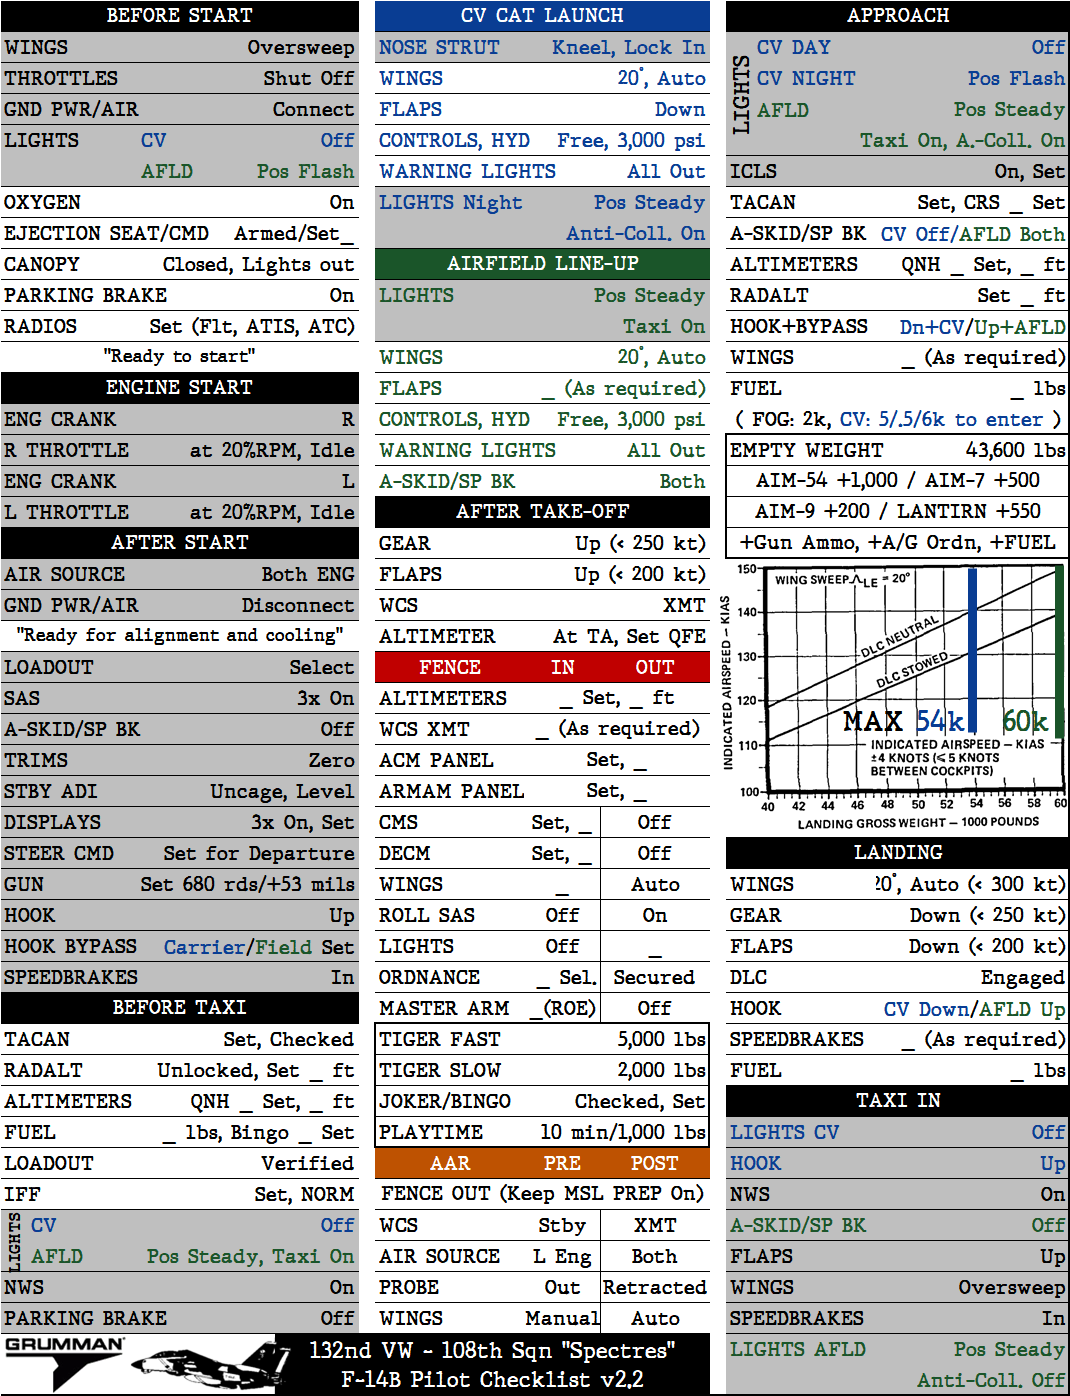
\includegraphics[width=\textwidth]{appendices/checklist-pilot}

\section{RIO CHECKLIST}

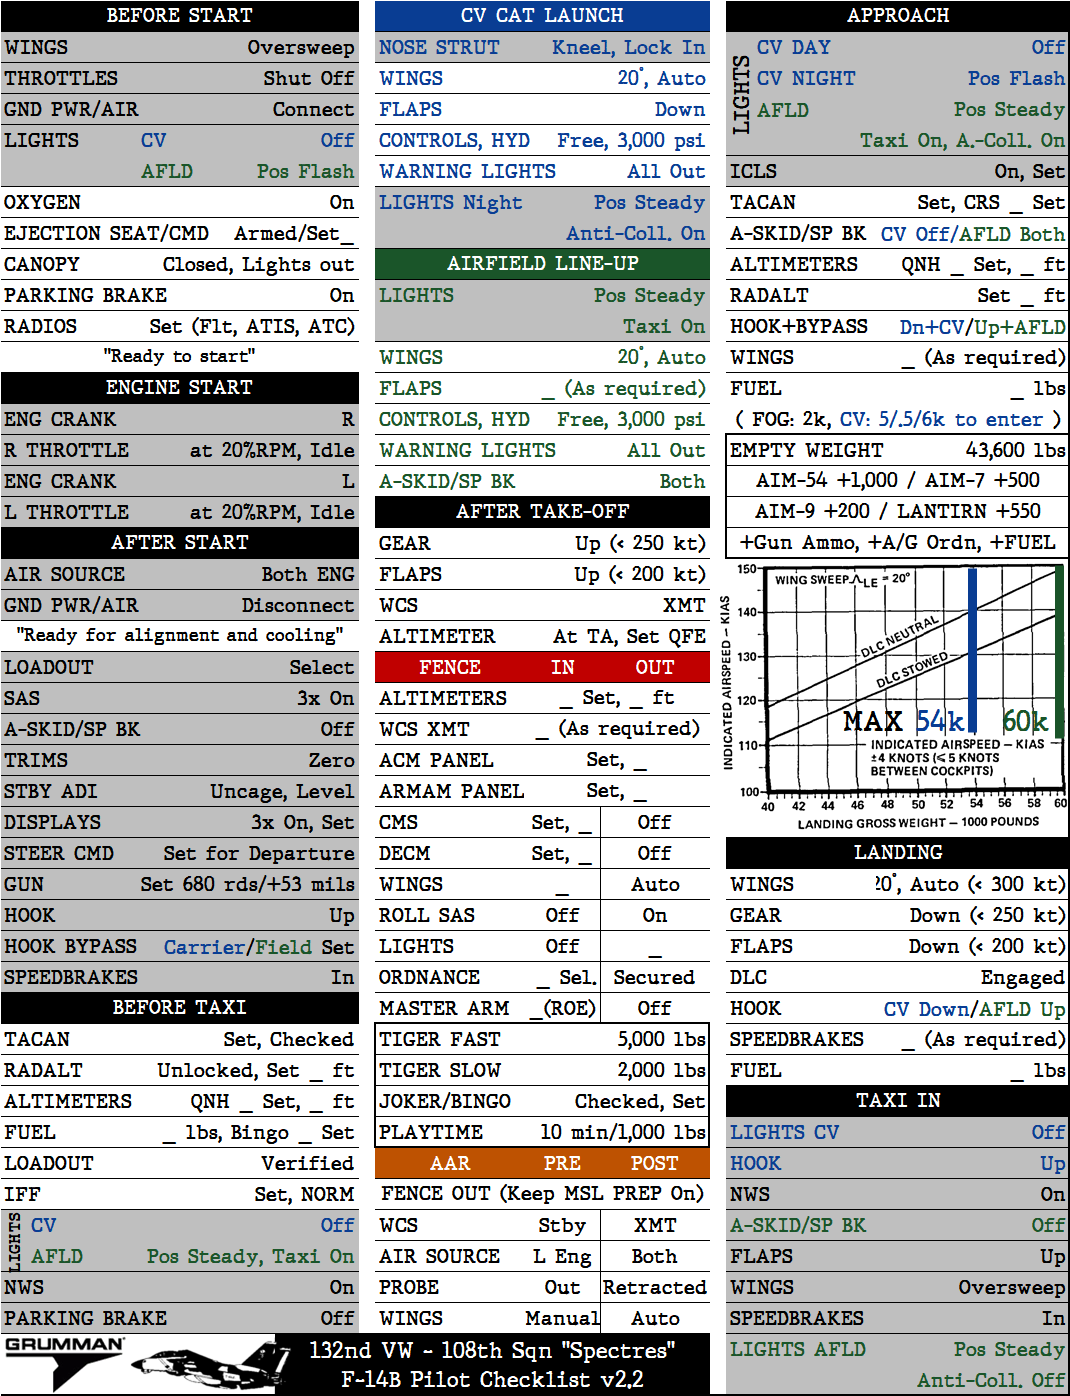
\includegraphics[width=\textwidth]{appendices/checklist-pilot}

\section{RADAR ELEVATION DATA}

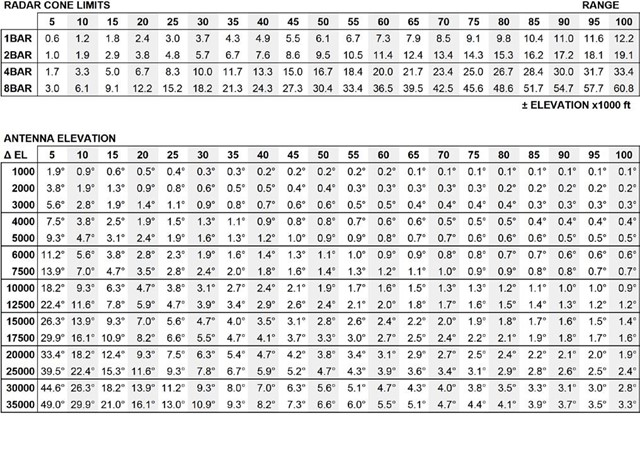
\includegraphics[width=\textwidth]{appendices/radar-elevation}

\section{FUEL / WEIGHT / SPEED DATA}

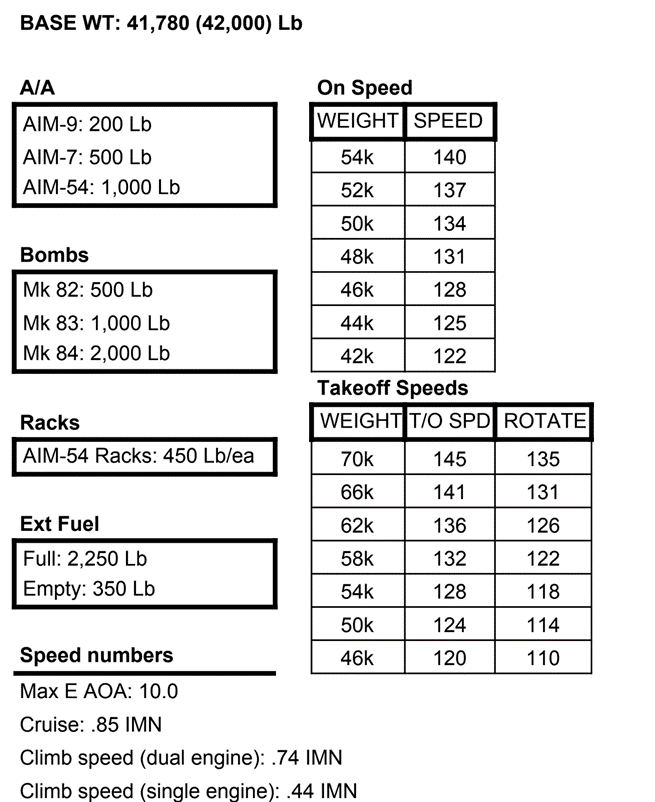
\includegraphics[width=\textwidth]{appendices/fuel-weight-speed}

\section{RADAR MATING}
\label{sec:radar-mating}

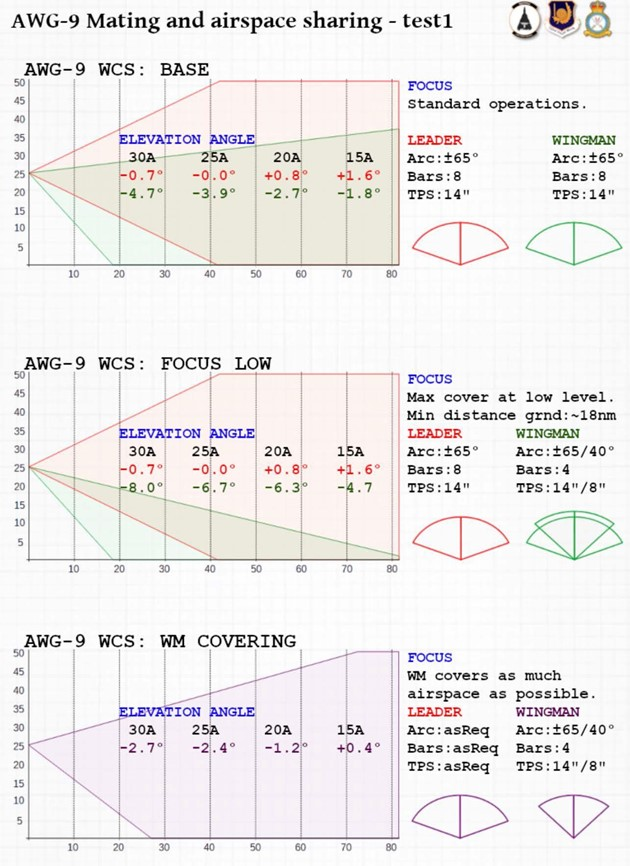
\includegraphics[width=\textwidth]{appendices/radar-mating}

\section{TCN UPDATE INS REFERENCE}

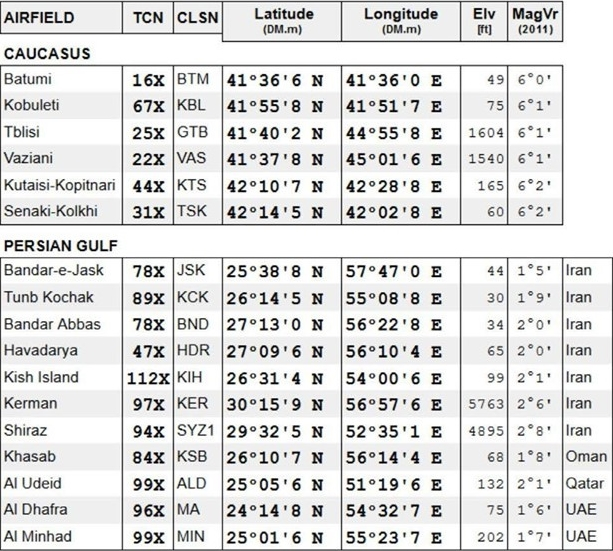
\includegraphics[width=\textwidth]{appendices/tacan-updates}

\subsection*{Process}

\begin{enumerate}
  \item Select a TACAN channel whose latitude and longitude correspond to an
    update point.

  \item Hook desired update point (WAYPT 1, FIX PT, HOME BASE, etc.)

  \item CATEGORY switch - NAV

  \item TACAN FIX button - Depress

  \item Observe present position delta readout

  \item If delta is unsatisfactory, deselect TACAN FIX and repeat steps 2
    through 7

  \item FIX ENABLE button - Depress
\end{enumerate}

\section{LIGHTING REFERENCE}%
\label{sec:appendix-lights}

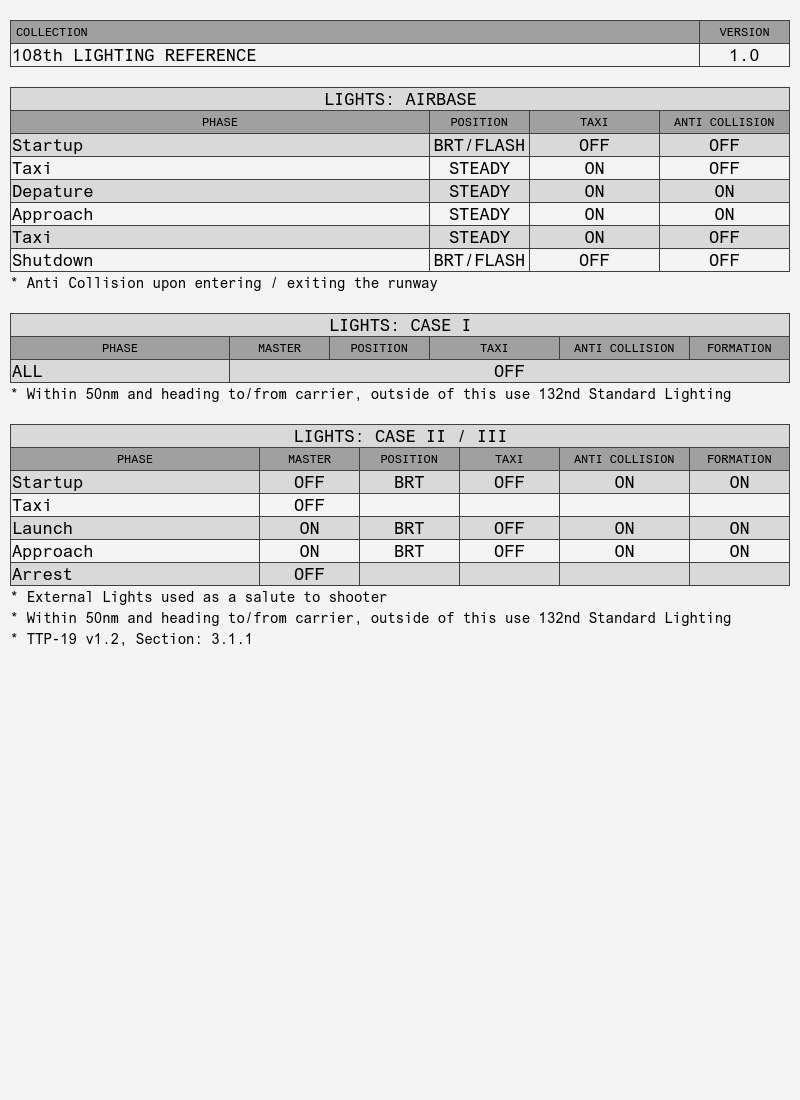
\includegraphics[width=\textwidth]{appendices/lighting}
